\section{Method}\label{sec:method}

% \subsection{Pipeline for Automatic TCT Screening}
% \label{section-3-1}
The overall TCT screening framework is presented in Fig. \ref{fig:overview}, which consists of three major steps in a hierarchical manner: 

\begin{figure*}[ht]
    \centering  
    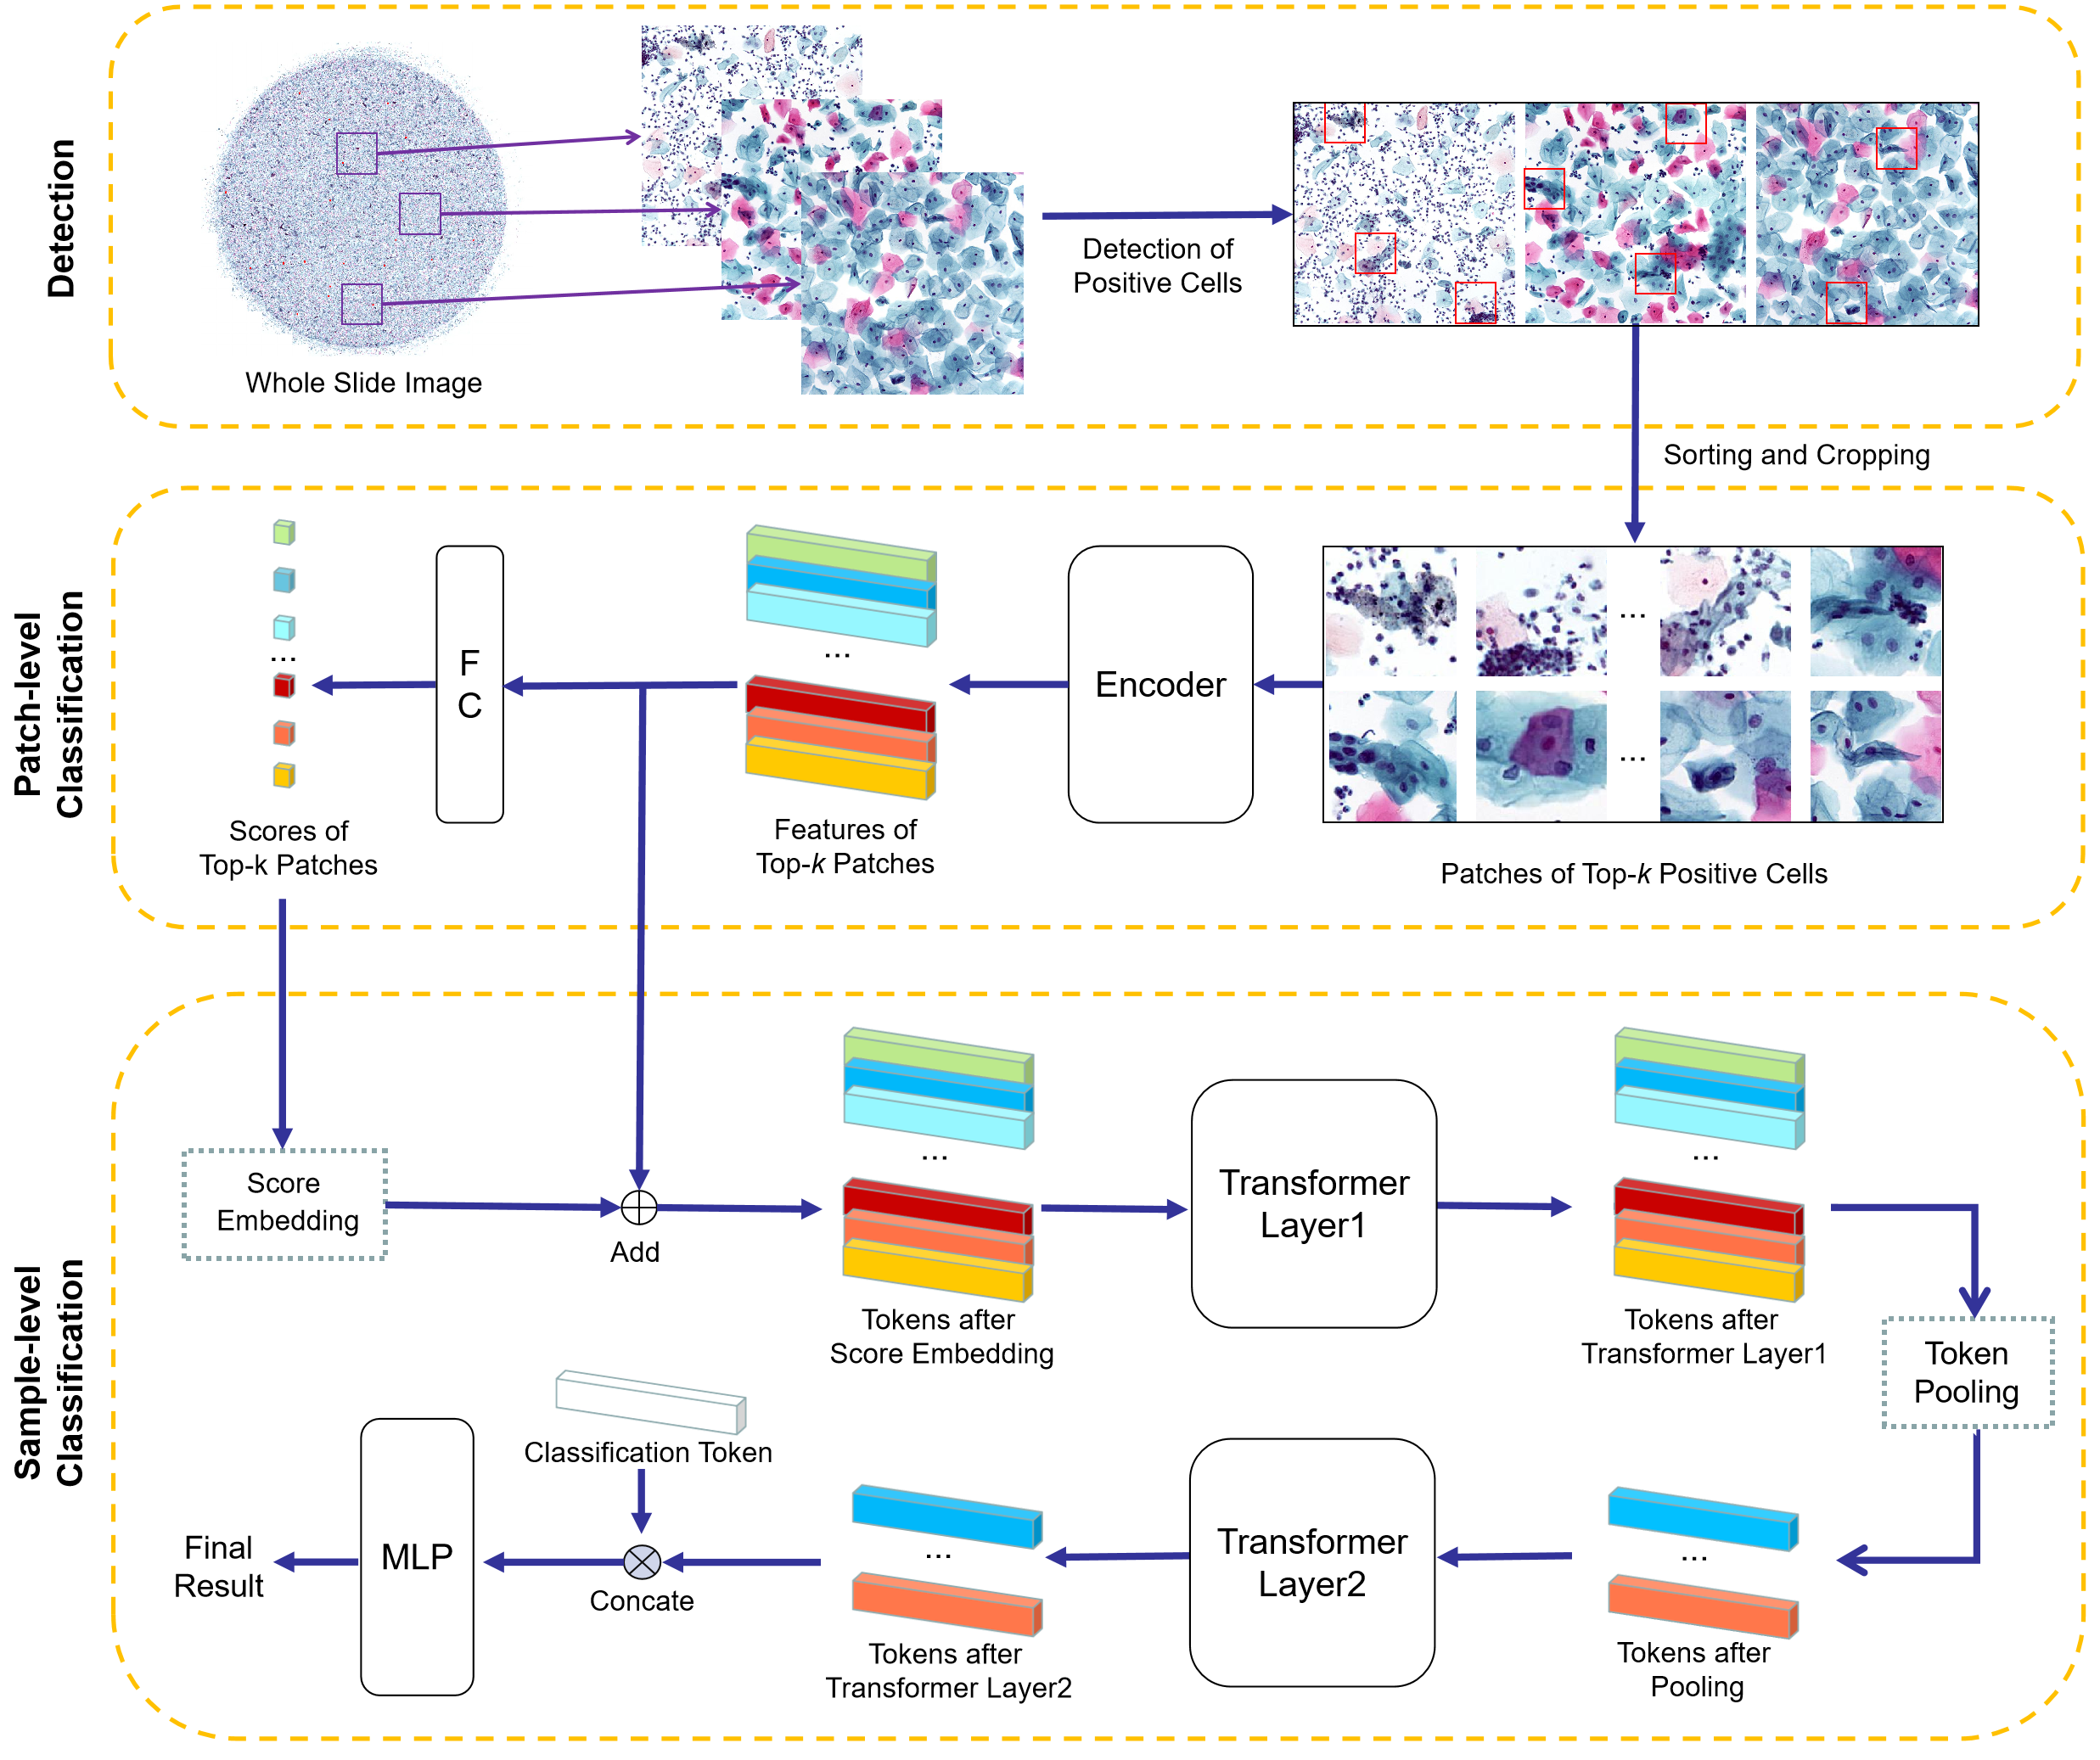
\includegraphics[width=\textwidth]{figures/pipeline.png}
    \caption{The overall pipeline of TCT screening, including the detection, patch-level classification and sample-level classification steps. The detection step intends to locate suspicious cervical cells, and extract their corresponding patches with the size of 224$\times$224. The patch-level classification step obtains the features and scores of the top $k$ patches with the highest possibility of abnormality, which are fed into score embedding and token pooling in transformer layers, and then concatenated with the classification token for passing through MLP to get the final result in the sample-level step.}
    \label{fig:overview}
\end{figure*}

\begin{itemize}
    \item 
    \textbf{Step 1:} We acquire the WSI data for each sample and conduct necessary quality control as well as pre-processing works. 
    Then, we apply an in-house cell detection network and identify those cells that are suspiciously positive (e.g., highlighted by red boxes \todo{They are not red enough in the figure} in the top row of Fig. \ref{fig:overview}). To ensure the feasibility of the detection process, every WSI sample is partitioned into a collection of tiled images sized 1024$\times$1024, which are used for suspicious cell detection separately. 
    % Besides, since the screening aims to pick up all samples that are eventually diagnosed as positive, the cell detection here usually works at high sensitivity, leading to many false positives in the detection outcomes from a very large WSI sample. 
    % Therefore, for each detected cell, we will perform patch-level classification in the second step to refine the detection result.
    \item 
    \textbf{Step 2:}  For each detected suspicious cell, we center-crop its corresponding patch (224$\times$224) to collect a patch-level cervical cell dataset. The patches in the dataset have been manually labeled by the pathologists and are used to train a binary classifier. Our aim is to use the classifier for false-negative suppression of the detected cells, which are also ranked based on the confidence score from the classifier. Here the top-$k$ (=20 in our implementation) cells with the highest scores are selected for the final sample-level diagnosis in Step 3. 
    \item 
    \textbf{Step 3:} We ensemble all top-$k$ patches via a transformer network to attain the sample-level classification. Particularly, we use the feature embedding from the patch-level classifier as the token for each cell patch, which is fed into the transformer. The transformer network is applied here to determine the contributions of individual patches dynamically, and group the tokens according to the intrinsic similarity among the patches. In this way, the feature representation after pooling becomes more effective to characterize the abnormality status of the WSI sample, leading to a more accurate sample-level diagnosis.
\end{itemize}

Note that our TCT screening system is not designed to depend on the specific detection method, and we also explore its feasibility by evaluating the effectiveness of three widely-applied detection models adopted in the pipeline, which are RetinaNet, FasterRCNN and Yolov3. Section \ref{section-3-2} and Section \ref{section-3-3} further illustrate the implementation details of the patch-level and sample-level classification steps, respectively.


\subsection{Patch-Level Classification}
\label{section-3-2}

% The patch-level classification deals with the patches centered on the suspicious cells that are previously detected. Since the cell detection is designed to be highly sensitive to avoid missing the potentially positive cells, the patch-level classification here is necessary to reduce the false positives in the detection results. 

% In order to make model have better feature representation and classification ability, we impose additional feature clustering constraints on the model based on the cross-entropy loss function. Furthermore, unlike the normal direct clustering constraint on each class, we take a selective cluster constraint on those patches which are a part of one batch. The process of different losses is shown in Figure \ref{fig:patch}.

We illustrate patch-level classification in Fig. \ref{fig:patch}.
Particularly, we use SEResNext50 as the backbone for the encoder. 
Individual patches pass through the convolutional layers, pooling layers, and a global average pooling (GAP) layer, to reach a 2048-dimensional feature space. 
The feature vector of each patch is further processed by a fully connected (FC) layer to yield the classification result. The classification network is further optimized by the cross-entropy-loss. 

\begin{figure*}[ht]
    \centering
    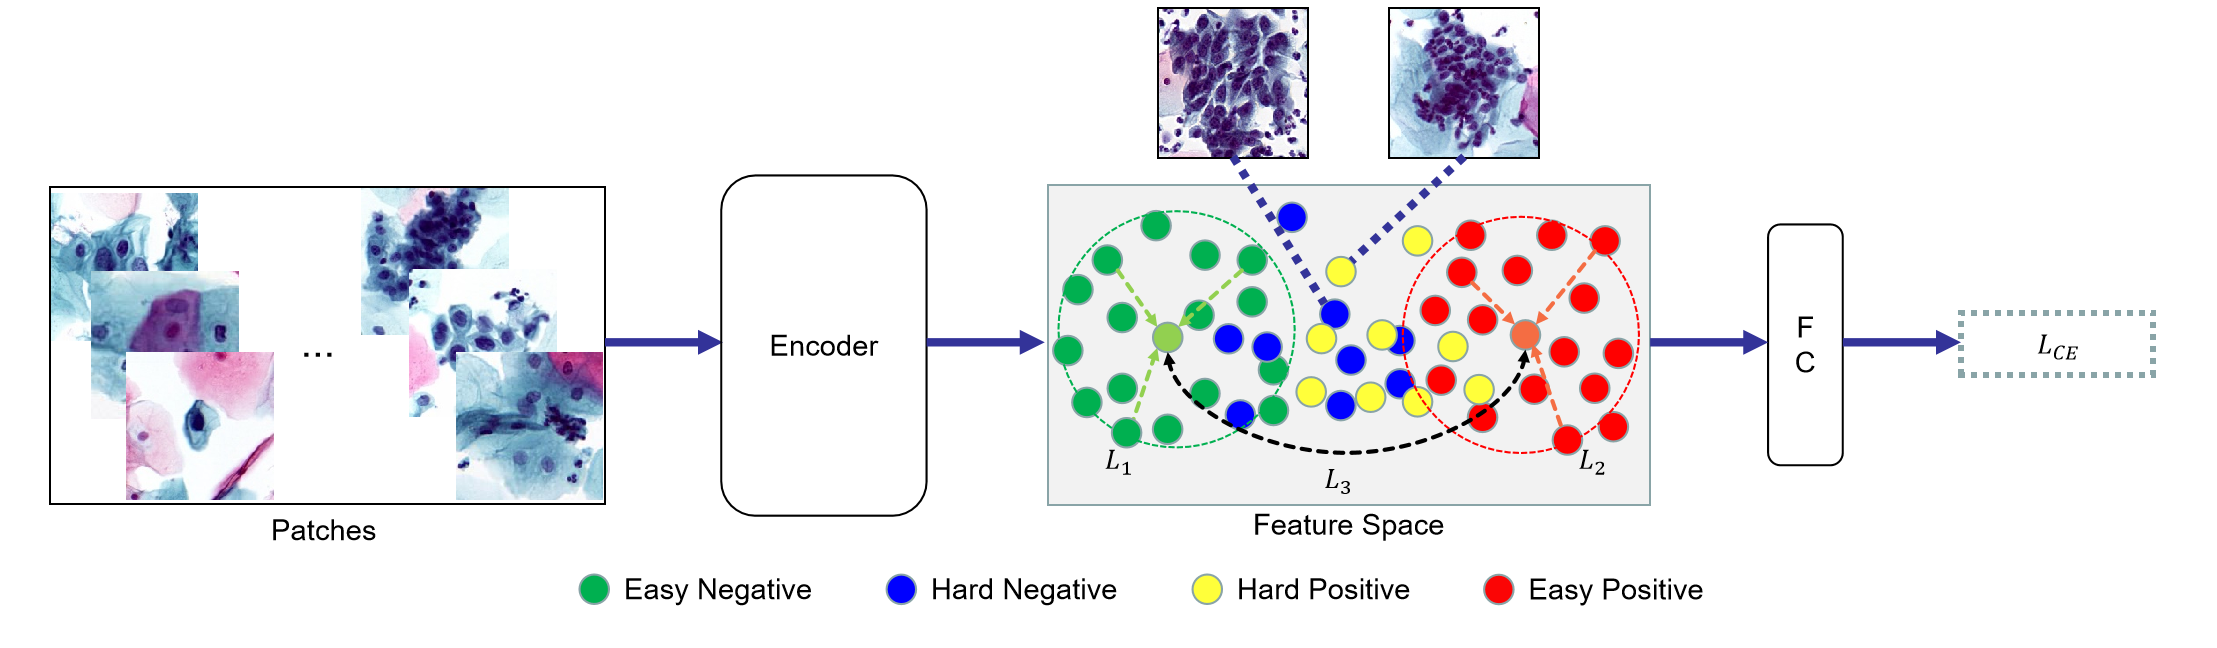
\includegraphics[width=\textwidth]{figures/patch-level.png}
    \caption{Diagram of our hard patch mining method on patch-level classification, the green points represent the features of easy negative patches(EN), blue points represent the features of hard negative patches(HN), yellow points represent the features of hard positive patches(HP), red points represent the features of easy positive patches(EP). Up of the feature space are two examples of HN and HP with similar appearance, of which left are normal cells, and the changes in cell morphology may be related to micro-adenogenesis, which is common in the late menstrual cycle of women taking oral contraceptives, and right are typical positive cells. We impose constraints on EN and EP which is ${L}_{1}$ and ${L}_{2}$ to make them closer to their respective cluster centers, and ${L}_{3}$ make features between different classes far away.}
    \label{fig:patch}
\end{figure*}
% However, as neglected by many conventional methods, the confusion about this classification task mostly originates from the hard patches, while the relatively easy patches can be well handled.
% Therefore, our patch-level classification model will emphasize the roles of those hard patches by referring to the data distribution in the latent feature space. 


It is non-trivial to tag a certain patch as positive or negative. 
There are hard patches, the labels of which have high uncertainty even for professional pathologists, which are shown in Fig. \ref{fig:patch}. 
In binary classification, simply calculating the cross-entropy loss cannot effectively separate those hard-positive and hard-negative patches. \todo{The motivations of why making these two extra labels unremain unclear to me.}
Therefore, we impose an additional constraint of hard-patch mining in patch-level classification.
With hard-patch mining, the easy-positive and easy-negative patches are pushed apart after they are embedded in the latent space. 
The hard samples can utilize the wide gap between the easy-positive and easy-negative patches for their distributions in the latent space.
In this way, our patch-level classification network is capable of better modeling the latent feature space, and distinguishing the positive/negative patches.

The hard patches are identified according to their contributions to computing the cross-entropy loss as in Fig. \ref{fig:patch}. 
In particular, we divide one batch of patches according to a certain threshold $m$ \todo{where is this $m$ coming from?} of the CE loss value of every patch in this batch (which we test with 0.3, 0.4, 0.5, 0.6, 0.7 in our experiment, and finally defined as 0.5 in our method), and divide them into easy patches (the loss value smaller than m) and hard patches (the loss value bigger than m).

We encourage the easy-negative and easy-positive to distribute compactly. 
To this end, we calculate the mean feature vectors for the easy-negative and easy-positive patches based on their feature embedding in the previous epoch. 
We denote the two mean feature vectors as $\bar{x}^e_{n}$ and $\bar{x}^e_{p}$, respectively.
Next, we calculate the cosine similarity between each patch in the current batch and the corresponding mean feature vector, which is a commonly used metric to measure the similarity between two vectors ~\cite{nguyen2010cosine}, \cite{zhang2022whole}, \cite{cao2022parallel}. Within the two groups of easy-positive and easy-negative, we define two losses:
\begin{equation}
    \begin{aligned}
        L_{1}&=1-\frac{1}{|\mathcal{B}^e_{n}|}\sum_{i \in {\mathcal{B}^e_{n}}}  S( x_{i},\bar{x}^e_{n} ).\\
        L_{2}&=1-\frac{1}{|\mathcal{B}^e_{p}|}\sum_{i \in {\mathcal{B}^e_{p}}}  S( x_{i},\bar{x}^e_{p} ).
    \end{aligned}
\end{equation}
Here, $\mathcal{B}^e_{n}$ and $\mathcal{B}^e_{p}$ indicate the current batches of the two groups of easy-positive and easy-negative. 
And the two losses encourage all easy patches to distribute compactly within their groups, implying more space is left for the hard patches in the latent space.
We further separate the EN and EP classes by introducing $L_{3}=S(\bar{x}^e_{n},\bar{x}^e_{p})$. In this way, the two classes can move apart from each other in the latent space.
\begin{figure*}[ht]
    \centering
    \includegraphics[scale=0.2]{figures/token.png}
    \caption{The similarity maps of the tokens, We selected three typical samples, namely, NILM, ASC-US and High-Level samples, the top 20 patches obtained from the detection network are as shown in the figure. The corresponding value of each patch is their score after passing through the patch-level classification network. The similarity map of the feature vectors obtained by encoding the 20 patches is on the right.}
    \label{fig:vit}
\end{figure*}
Finally, we derive the overall clustering loss:
\begin{equation}
L_{p}=L_{ce}+L_{1} + L_{2} + L_{3}.
\end{equation}
The first term $L_{ce}$ is the cross-entropy loss for the classification. And the rest three terms ($L_{1}$, $L_{2}$, $L_{3}$) are for the hard-mining loss.
In this way, we expect the intra-class feature encoding of the easy patches to be relatively similar, while the inter-class feature encoding should be far away. 
With the constraint encoding of the easy patch feature vector, the feature encoding of the hard patch will also gradually be different, which will increase the feature space encoding ability of the patch-level classification model.




%In order to enhance the interpretability of our method, we visualize the token correlation, and we select three typical samples, NILM, ASC-US and a high-level, which NILM is the negative sample and ASC-US, high-level is the positive sample. The first column shows the original pictures of one sample, which consists of 20 patches, and each patch is 224*224 in size. The second column shows the correlation between 20 tokens, these tokens have obvious characteristics of aggregation, which means that if we directly use 20 tokens for operation, a lot of redundant information will be generated, and there are not always only two types of clusters, so an arbitrary number of cluster centers The clustering algorithm is necessary. The third and fourth columns show the importance of the classification token. As shown in the figure, the token that contributes more to the classification token has a darker color. The visualization results show that our method can effectively integrate the key The token is extracted from a bunch of tokens.

\subsection{Sample-level Classification}
\label{section-3-3}

The sample-level classification relies on the top-\textit{k} suspicious patches, which is illustrated at the bottom of Fig. \ref{fig:overview}. 
We input the top-\textit{k} patches into the transformer network. 
Specifically, we use the feature vector in the latent space before the FC layer of the patch-level classifier as the token of each input patch.
The network has two transformer layers, the input dimensions of both transformer layers are 2048, and their depths are 8 and 4 respectively. 
% Since there are often some patches in multiple patches whose feature expressions are very similar, the transformer network structure needs to integrate the feature information of the top k to further extract the global feature information from them, and finally get a classification result of the whole sample. 

% The patch-level classification provides scores, rather than only binary outcomes, to allow us to rank the patches according to their likelihood of being positive. 
% Specifically, we pick up the top-\textit{k} patches, and feed them to the transformer based on their latent representation extracted by the patch-level classification network. 
% The transformer architecture can integrate those \textit{k} patches and reach a global representation of the whole WSI.

Particularly, In order to better transfer the independent information of each patch to the model, similar to position embedding in Vision in Transformer (ViT)\cite{dosovitskiy2020image}, we propose score embedding to input the score of each patch in the patch level classification model into the transformer layer. Next, according to our observation in Fig. \ref{fig:vit}, many features of different patches are redundant, so we used the token pooling strategy to help the model filter redundant feature expressions. The specific methods of score embedding and token pooling are as follows.



\subsubsection{Score Embedding}
Preserving the independent information of each part of a whole has been proven to be an effective method in the field of deep learning, such as patch position embedding in an image\cite{dosovitskiy2020image}, word position embedding in language text\cite{vaswani2017attention}, and graph embedding in recommendation system\cite{goyal2018graph}, 
The abnormality can occur in anywhere of the WSI. 
How to effectively embed information on cells in different patches of images so that the model can make full use of this information and make different patches have independent information expression will become a problem to be solved\todo{I don't understand this sentence. What is independent information?}. Although WSI images, like those in vit, are divided into many small patches, since WSI images are processed after uniform centrifugation, the location information of each patch is no longer meaningful. So we use score embedding instead of position embedding to solve this problem.



We choose the classification score obtained by using the feature vector of each patch through the fully connected layer of the classification model at the patch level as the location information of the feature space for feature space location embedding, which is shown in Figure\ref{fig:overview}. 
We expand these scores to the same shape as features on the channel dimension, which is 2048 dimensions, and add them to the original features to get a new set of features.
This strategy is very simple but effective. It can maintain the independent information of each patch image when the location information cannot be used, so as to improve the classification accuracy.


\subsubsection{Token Pooling}
To observe whether the features input to the transformer layer is valid, we calculate the similarity map for all features of the top k patches of a sample. As shown in the figure\ref{fig:vit}, we sort each patch from small to large according to its classification score. The similarity map also follows this sort. It can be seen that in some samples, such as a) NILM, many patch features have strong similarities. In addition, among the top k patches of different samples, the degree of similarity of tokens is also different. The k pictures of negative samples tend to have similar features, while the k pictures of positive samples show a group-by-group approach, but the number of groups is often uncertain.
So in order to use tokens more concisely and efficiently, we use the token pooling method to reduce redundant tokens to highlight important tokens, so that the model can better adapt to the task of negative and positive classification.


Due to the uncertainty of the number of groupings, we generally refer to the affinity promotion (AP)\cite{frey2007clustering} algorithm to perform the token pooling operation. The AP algorithm updates the attractiveness and attribution information of each point in the similarity matrix, and adds the attractiveness and attribution after reaching the preset number of iterations to obtain the cluster center. Specifically, in our proposed method, after obtaining the features after score embedding, we first use a transformer layer to calculate the self-attributes of these features. After obtaining a group of new features, we use the AP algorithm to cluster these features. After obtaining n-class features, we perform average pooling operations on these n-class features to obtain more concise feature expression after aggregation.


In addition, since we need to unify the number of tokens in the same batch, we use a small trick, which will find the sample with the largest number of tokens in the current batch, and align the tokens of other samples with it by filling zero with it. 

Later, we again calculate the self-attention of these simplified features through another transformer layer, and splice a learnable classification token with it. Finally, the final classification result is obtained after the MLP module.